\chapter{Fundamentação Teórica}
\label{cap:fundamentacao-teorica}

Este capítulo apresenta os fundamentos conceituais e tecnológicos relacionados ao desenvolvimento da plataforma ``Sobral em Mapas''. Inicialmente, são abordados os Sistemas de Informação Geográfica (SIG), as aplicações WebGIS e os padrões de interoperabilidade geoespacial, com destaque para os serviços WMS, WFS e WMTS. Em seguida, são discutidos conceitos de arquitetura de software e as tecnologias empregadas na solução, incluindo React, Leaflet, React-Leaflet, Laravel, MySQL e GeoServer. Por fim, são apresentados os fundamentos da conteinerização, da computação em nuvem, da responsividade e da usabilidade, seguidos de uma análise de trabalhos relacionados que contribuem para contextualizar a proposta desenvolvida.


\section{Sistemas de Informação Geográfica}
\label{sec:sig}


Os Sistemas de Informação Geográfica (SIG), conhecidos em inglês como \textit{Geographic Information Systems} (GIS), podem ser definidos como sistemas computacionais utilizados para armazenar, organizar, manipular, analisar e representar informações associadas a posições geográficas \cite{Silva2013}. \glsunset{SIG}\glsunset{GIS}

A utilização de informações georreferenciadas permite estabelecer relações entre diferentes conjuntos de dados e identificar padrões que poderiam ser menos evidentes quando analisados apenas por meio de tabelas ou documentos textuais. Entre as operações normalmente associadas aos \gls{SIG} encontram-se a consulta espacial, a sobreposição de camadas, a identificação de feições e a realização de medições, tornando essas ferramentas relevantes tanto para atividades técnicas quanto para processos de planejamento e gestão territorial.



\subsection{Dados Vetoriais e Matriciais}
\label{sec:dados-geoespaciais}

Os dados geográficos podem ser representados principalmente por meio de modelos vetoriais e matriciais. No modelo vetorial, os elementos geográficos são descritos utilizando pontos, linhas e polígonos. Os pontos são empregados na representação de elementos cuja localização é mais relevante que sua extensão, como escolas e unidades de saúde; as linhas podem representar vias, redes e trajetos; enquanto os polígonos permitem delimitar bairros, áreas administrativas e outras regiões territoriais. Além da geometria, as feições vetoriais podem possuir atributos descritivos associados, como nome, endereço e categoria, possibilitando relacionar características específicas aos elementos representados.

A representação dessas geometrias baseia-se na organização de coordenadas espaciais, interpretadas conforme um sistema de referência. Um ponto pode ser definido por um par de coordenadas, como longitude e latitude, enquanto as linhas são formadas por sequências de posições conectadas. Os polígonos, por sua vez, utilizam sequências de coordenadas que delimitam contornos fechados, permitindo representar a extensão de determinada área geográfica. Essas estruturas podem ser armazenadas em formatos vetoriais, como o GeoJSON, que organiza geometrias e atributos descritivos em uma representação estruturada, facilitando seu intercâmbio entre aplicações e serviços geoespaciais \cite{RFC7946}.

O modelo matricial, também denominado \textit{raster}, representa o espaço por meio de uma matriz de células ou pixels, aos quais são associados valores referentes às características da área representada. Imagens de satélite, fotografias aéreas e modelos digitais de elevação constituem exemplos desse tipo de representação. Em aplicações geográficas, os modelos vetorial e matricial são frequentemente utilizados de maneira complementar, permitindo combinar mapas de base matriciais com camadas temáticas referentes a equipamentos públicos, limites territoriais ou redes de transporte. A Figura \ref{fig:dados-vetoriais-matriciais} apresenta uma comparação entre essas formas de representação.

\begin{figure}[htb]
    \centering
    \caption{Representação dos modelos de dados vetoriais e matriciais}
    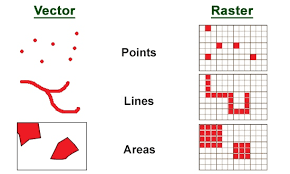
\includegraphics[width=0.70\textwidth]{figuras/dados-vetoriais-matriciais.png}
    \label{fig:dados-vetoriais-matriciais}
    \fonte{Imagem disponibilizada em \citeonline{Yusuf2016}.}
\end{figure}


\subsection{Sistemas de Referência Espacial}
\label{sec:sistemas-referencia}

Para que dados provenientes de diferentes fontes possam ser apresentados corretamente em uma mesma visualização cartográfica, é necessário estabelecer como suas coordenadas correspondem à superfície terrestre. Os sistemas de referência espacial definem os parâmetros utilizados para interpretar essas coordenadas, considerando aspectos como o sistema de coordenadas, o datum geodésico e, quando aplicável, a projeção cartográfica. Nos sistemas de coordenadas geográficas, as posições são expressas por latitude e longitude, geralmente em graus, enquanto os sistemas projetados utilizam coordenadas planas, frequentemente representadas em metros \cite{QGISCoordenadas2025}. A Figura \ref{fig:coordenadas-geograficas} ilustra a organização das coordenadas geográficas a partir dos paralelos e meridianos terrestres.

\begin{figure}[htb]
    \centering
    \caption{Representação das coordenadas geográficas de latitude e longitude}
    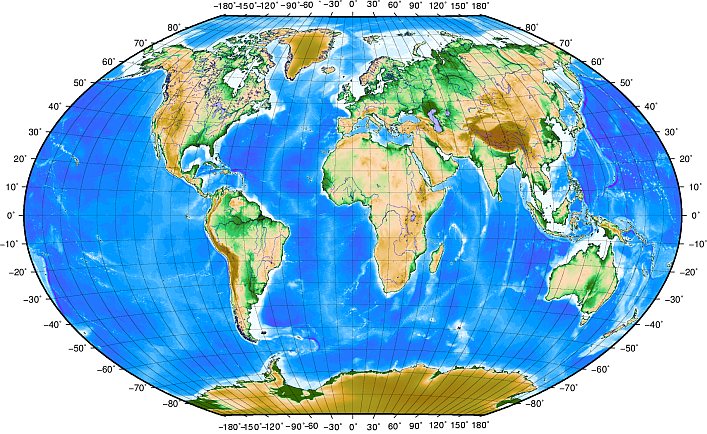
\includegraphics[width=0.70\textwidth]{figuras/coordenadas-geograficas.png}
    \label{fig:coordenadas-geograficas}
    \fonte{Imagem disponibilizada em \citeonline{QGISCoordenadas2025}.}
\end{figure}

Quando referências espaciais distintas não são consideradas adequadamente, camadas que representam uma mesma região podem apresentar deslocamentos ou incompatibilidades. Nesse contexto, a identificação dos sistemas de referência e, quando necessário, a transformação de coordenadas são fundamentais para garantir o alinhamento das informações. Em aplicações \gls{WebGIS}, bibliotecas cartográficas e servidores de mapas precisam interpretar corretamente essas referências, permitindo que dados provenientes de diferentes fontes sejam sobrepostos de maneira consistente.

\section{Sistemas de Informação Geográfica na Web}
\label{sec:webgis}

O avanço das tecnologias de Internet e dos navegadores possibilitou a disponibilização de funcionalidades geográficas diretamente na web, consolidando os Sistemas de Informação Geográfica na Web, conhecidos como WebGIS \cite{Silva2013}. \glsunset{WebGIS} Essas aplicações permitem acessar mapas e informações espaciais por meio de navegadores, sem exigir a instalação de programas especializados, oferecendo recursos como navegação cartográfica, alteração do nível de \textit{zoom}, ativação de camadas temáticas e consulta de informações geográficas.

As plataformas \gls{WebGIS} não substituem os programas tradicionais de geoprocessamento, que permanecem relevantes para atividades especializadas de edição, produção cartográfica e análise espacial. Sua principal contribuição está na ampliação do acesso e do compartilhamento das informações geográficas \cite{BastosCamboim2022}. Além disso, essas plataformas podem distribuir responsabilidades entre diferentes componentes, de modo que o armazenamento e a publicação dos dados sejam realizados no ambiente servidor, enquanto a visualização cartográfica e as interações com a interface ocorrem no navegador do usuário \cite{VinuezaMartinez2024}.

\subsection{WebGIS na Gestão Pública}
\label{sec:webgis-gestao-publica}

Na Administração Pública, as aplicações \gls{WebGIS} permitem reunir informações relacionadas à mobilidade urbana, à saúde, à educação, à infraestrutura e à organização territorial em uma interface cartográfica comum. Essa integração pode apoiar atividades de consulta e planejamento municipal, além de ampliar o acesso às informações geográficas por cidadãos, estudantes, pesquisadores e profissionais interessados no território \cite{Alcantara2015,Marotta2020}.

Entretanto, a utilidade dessas plataformas depende não apenas das funcionalidades disponibilizadas pela interface, mas também da qualidade e da atualização das bases geográficas, da consistência dos metadados e da disponibilidade dos serviços responsáveis pelo fornecimento das informações. Nesse contexto, a organização dos dados e a interoperabilidade entre os componentes constituem aspectos fundamentais para garantir a continuidade e a confiabilidade das informações apresentadas.



\section{Interoperabilidade e Padrões Geoespaciais}
\label{sec:interoperabilidade}

Uma plataforma geográfica pode integrar diferentes ferramentas responsáveis pelo armazenamento, processamento e visualização das informações espaciais, tornando necessários mecanismos de interoperabilidade entre seus componentes. Nesse contexto, o \textit{Open Geospatial Consortium} (OGC) desenvolve padrões que permitem a comunicação entre servidores, clientes cartográficos e ferramentas de geoprocessamento, reduzindo a dependência entre tecnologias específicas \cite{OGCWMS,OGCWFS,OGCWMTS}. \glsunset{OGC} Entre os principais serviços padronizados pelo \gls{OGC}, destacam-se o WMS, o WFS e o WMTS, que apresentam diferentes formas de disponibilização das informações geoespaciais.

\subsection{Web Map Service}
\label{sec:wms}

O \textit{Web Map Service} (WMS) estabelece uma interface padronizada para obtenção de representações cartográficas produzidas por servidores de mapas \cite{OGCWMS}. \glsunset{WMS} Por meio da operação \texttt{GetMap}, o cliente solicita camadas geográficas, informando parâmetros como extensão territorial, dimensões da imagem, sistema de referência e formato de saída, geralmente \texttt{PNG} ou \texttt{JPEG}. Entre esses parâmetros, a \texttt{BBOX} (\textit{Bounding Box}) delimita a área geográfica solicitada. Diferentemente de serviços que disponibilizam as feições completas, o \gls{WMS} fornece principalmente sua representação visual, permitindo que dados originalmente vetoriais sejam processados e apresentados como imagens cartográficas.

\subsection{Web Feature Service e GeoJSON}
\label{sec:wfs}

O \textit{Web Feature Service} (WFS) permite acessar diretamente feições geográficas e seus atributos, diferentemente do \gls{WMS}, que disponibiliza principalmente representações cartográficas \cite{OGCWFS}. \glsunset{WFS} Dessa forma, pontos, linhas e polígonos podem ser consultados e transferidos ao cliente para operações de seleção, filtragem e análise espacial. Entre os formatos utilizados para representar essas informações encontra-se o \texttt{GeoJSON}, padronizado pelo RFC 7946, que emprega a estrutura \gls{JSON} para organizar geometrias e atributos descritivos \cite{RFC7946}. Entretanto, o \texttt{GeoJSON} constitui um formato de dados, e não um serviço geoespacial, podendo ser utilizado independentemente ou como resposta de determinadas implementações de \gls{WFS}.

\subsection{Web Map Tile Service}
\label{sec:wmts}

O \textit{Web Map Tile Service} (WMTS) disponibiliza representações cartográficas organizadas em mosaicos de imagens, denominados \textit{tiles}, distribuídos em matrizes associadas a níveis de escala predefinidos \cite{OGCWMTS}. \glsunset{WMTS} Essa organização permite solicitar apenas os mosaicos necessários à área visualizada, favorecendo o armazenamento e o reaproveitamento das imagens por mecanismos de \textit{cache}. Diferentemente do \gls{WMS}, que permite solicitar representações para extensões geográficas arbitrárias, o \gls{WMTS} utiliza matrizes e níveis de escala padronizados, facilitando a reutilização dos mosaicos cartográficos.

A Tabela \ref{tab:comparativo-ogc} sintetiza as principais características dos serviços apresentados.

\begin{table}[!htbp]
    \captionsetup{width=15cm}
    \Caption{\label{tab:comparativo-ogc} Comparativo entre serviços geoespaciais}
    \IBGEtab{}{
        \begin{tabular}{p{3.0cm}p{3.6cm}p{3.6cm}p{3.6cm}}
            \toprule
            \textbf{Característica} & \textbf{WMS} & \textbf{WFS} & \textbf{WMTS} \\
            \midrule \midrule

            Conteúdo fornecido &
            Imagens cartográficas &
            Feições e atributos &
            Mosaicos de imagens \\
            \midrule

            Geometrias disponíveis &
            Não diretamente &
            Sim &
            Não diretamente \\
            \midrule

            Forma de consulta &
            Área geográfica e camadas &
            Feições e filtros &
            Matrizes e níveis de escala \\
            \midrule

            Processamento &
            Renderização no servidor &
            Processamento também no cliente &
            Mosaicos e mecanismos de cache \\
            \midrule

            Aplicações comuns &
            Camadas temáticas &
            Consulta de dados vetoriais &
            Mapas de base e mosaicos \\

            \bottomrule
        \end{tabular}
    }{
        \fonte{Elaborado pelo autor.}
    }
\end{table}

Embora esses padrões ofereçam diferentes formas de acesso às informações geográficas, o ``Sobral em Mapas'' utiliza principalmente o \gls{WMS} para consumir as camadas temáticas publicadas pelo GeoServer. O formato \texttt{GeoJSON}, por sua vez, é empregado na representação do limite territorial do município, sem a necessidade de utilização do \gls{WFS} na implementação desenvolvida.


\section{Arquitetura de Software em Aplicações Web}
\label{sec:arquitetura-software}

A arquitetura de software estabelece a organização dos principais componentes de um sistema, definindo suas responsabilidades e formas de comunicação \cite{Bass2021}. Essas decisões influenciam aspectos como manutenção, evolução, implantação e integração, sendo necessário considerar as características e os requisitos de cada aplicação na escolha da abordagem arquitetural.

\subsection{Arquitetura Monolítica e Arquitetura Desacoplada}
\label{sec:arquiteturas-web}

Na arquitetura monolítica, os diferentes módulos do sistema são reunidos em uma aplicação principal, geralmente desenvolvida e implantada como uma unidade. Essa abordagem pode simplificar a organização inicial de projetos menores, pois concentra funcionalidades e reduz a necessidade de comunicação entre serviços independentes. Entretanto, conforme a aplicação cresce, o aumento das dependências internas pode dificultar determinadas alterações e processos de implantação.

A arquitetura desacoplada, por sua vez, distribui responsabilidades entre componentes que se comunicam por interfaces bem definidas. Em aplicações web, essa separação ocorre frequentemente entre o \textit{front-end}, responsável pela interface e interação com o usuário, e o \textit{back-end}, que concentra regras de negócio, persistência e segurança. Em sistemas geoespaciais, essa organização pode incluir um servidor de mapas, responsável pela publicação das informações cartográficas.

A separação das responsabilidades pode favorecer a manutenção e a evolução dos componentes, desde que os contratos de comunicação sejam preservados. Por outro lado, exige maior atenção à configuração e à integração entre os serviços. A Tabela \ref{tab:comparativo-arquitetura} apresenta uma comparação entre as duas abordagens.

\begin{table}[htb]
    \captionsetup{width=15cm}
    \Caption{\label{tab:comparativo-arquitetura} Comparação entre arquitetura monolítica e desacoplada}
    \IBGEtab{}{
        \begin{tabular}{p{3.0cm}p{5.1cm}p{5.1cm}}
            \toprule
            \textbf{Característica} &
            \textbf{Monolítica} &
            \textbf{Desacoplada} \\
            \midrule \midrule

            Organização &
            Componentes reunidos em uma aplicação &
            Responsabilidades distribuídas entre componentes \\
            \midrule

            Implantação &
            Geralmente realizada como uma unidade &
            Pode ocorrer de forma independente \\
            \midrule

            Comunicação &
            Predominantemente interna &
            Realizada por interfaces e protocolos \\
            \midrule

            Manutenção &
            Alterações podem envolver diferentes módulos &
            Favorece a separação das modificações \\
            \midrule

            Infraestrutura &
            Pode apresentar menor complexidade inicial &
            Pode exigir maior configuração e integração \\

            \bottomrule
        \end{tabular}
    }{
        \fonte{Elaborado pelo autor.}
    }
\end{table}

\subsection{Single Page Application}
\label{sec:spa}

Uma \textit{Single Page Application} (SPA) é uma abordagem de desenvolvimento na qual a aplicação carrega inicialmente sua estrutura principal e atualiza dinamicamente partes da interface, sem exigir o recarregamento completo da página a cada interação. \glsunset{SPA} Esse comportamento permite construir interfaces interativas, nas quais diferentes componentes podem apresentar informações e responder às ações dos usuários de maneira integrada.

Em aplicações cartográficas, a utilização de uma \gls{SPA} permite manter o mapa, os painéis e as ferramentas ativos enquanto camadas e informações são atualizadas. Entretanto, essa abordagem não elimina a comunicação com o servidor, pois a aplicação continua realizando requisições para recuperar dados, autenticar usuários e executar operações relacionadas às regras de negócio.

\subsection{APIs e Arquitetura REST}
\label{sec:api-rest}

A comunicação entre componentes de uma arquitetura desacoplada pode ocorrer por meio de Interfaces de Programação de Aplicações (APIs), que estabelecem operações e contratos para a troca de informações entre sistemas. Em aplicações web, essa comunicação utiliza frequentemente o protocolo \gls{HTTP} e formatos estruturados, como \gls{JSON}, permitindo que diferentes tecnologias compartilhem dados por interfaces padronizadas.

O \textit{Representational State Transfer} (REST) é um estilo arquitetural para sistemas distribuídos apresentado por \citeonline{Fielding2000}. \glsunset{REST} Entre seus princípios destacam-se a separação entre cliente e servidor, a identificação de recursos e a comunicação sem a manutenção obrigatória de estado de sessão entre as requisições. Esses princípios orientam a organização de APIs voltadas à manipulação e à consulta de recursos.

Nas APIs baseadas em \gls{HTTP}, métodos como \texttt{GET}, \texttt{POST}, \texttt{PUT}, \texttt{PATCH} e \texttt{DELETE} são utilizados para representar diferentes operações. As respostas também empregam códigos de estado, sendo a família \texttt{2xx} associada geralmente ao sucesso da solicitação, \texttt{4xx} a problemas relacionados à requisição ou ao acesso, e \texttt{5xx} a falhas no processamento pelo servidor.


\section{Tecnologias de Desenvolvimento da Plataforma}
\label{sec:tecnologias}

O desenvolvimento de uma plataforma \gls{WebGIS} envolve tecnologias responsáveis pela interface cartográfica, pelo processamento das requisições, pelo armazenamento das informações administrativas e pela publicação dos dados geoespaciais. Esta seção apresenta as principais ferramentas relacionadas a essas responsabilidades.

\subsection{React, Leaflet e React-Leaflet}
\label{sec:frontend-tecnologias}

React é uma biblioteca JavaScript utilizada na construção de interfaces baseadas em componentes reutilizáveis \cite{ReactDocs}. Essa abordagem permite organizar funcionalidades e gerenciar estados da aplicação, como camadas selecionadas, painéis abertos e informações do usuário. Para a visualização cartográfica, Leaflet disponibiliza recursos de navegação, gerenciamento de camadas, representação de geometrias e integração com serviços geoespaciais, incluindo o \gls{WMS} \cite{LeafletDocs}. O React-Leaflet, por sua vez, integra esses recursos aos componentes React, permitindo controlar elementos do mapa por meio dos estados da aplicação \cite{ReactLeafletDocs}. Essa integração também pode ser ampliada com extensões destinadas a desenhos, medições e outras interações cartográficas.

\subsection{Laravel, Eloquent e Laravel Sanctum}
\label{sec:backend-tecnologias}

Laravel é um \textit{framework} PHP que oferece recursos para organização de aplicações web, incluindo rotas, validação, autenticação e acesso a bancos de dados \cite{LaravelDocs8}. Além de aplicações tradicionais, permite desenvolver APIs destinadas à comunicação com interfaces independentes, mantendo o processamento das regras de negócio no servidor.
O Eloquent é o mecanismo de Mapeamento Objeto-Relacional do Laravel, responsável por representar tabelas e relacionamentos do banco de dados por meio de modelos \cite{LaravelEloquent8}. Complementarmente, Laravel Sanctum fornece mecanismos de autenticação para aplicações e APIs, incluindo o uso de \textit{tokens} associados aos usuários \cite{LaravelSanctum8}. Em conjunto com as regras de autorização implementadas no servidor, esses recursos permitem controlar o acesso às funcionalidades administrativas.

\subsection{Banco de Dados MySQL}
\label{sec:mysql}

MySQL é um Sistema Gerenciador de Banco de Dados Relacional que organiza informações em tabelas relacionadas por chaves primárias e estrangeiras \cite{MySQL80}. Em uma plataforma \gls{WebGIS}, pode armazenar usuários, perfis, categorias, subcategorias e metadados das camadas, enquanto os dados geográficos podem permanecer em fontes externas especializadas. Essa separação distingue a persistência administrativa da publicação cartográfica.

\subsection{GeoServer}
\label{sec:geoserver}

GeoServer é um servidor de mapas de código aberto que permite publicar informações geoespaciais por meio de padrões interoperáveis, como \gls{WMS} e \gls{WFS} \cite{GeoServerDocs}. Sua utilização separa a disponibilização cartográfica das operações administrativas da aplicação, permitindo que a API gerencie usuários e metadados enquanto os serviços geoespaciais fornecem as camadas. Quando essa infraestrutura é externa, a integração depende da disponibilidade e da configuração dos recursos publicados.

A Tabela \ref{tab:responsabilidades-tecnologias} sintetiza as responsabilidades das principais tecnologias apresentadas.

\begin{table}[!htbp]
    \captionsetup{width=15cm}
    \Caption{\label{tab:responsabilidades-tecnologias} Principais tecnologias e responsabilidades em uma arquitetura WebGIS}
    \IBGEtab{}{
        \begin{tabular}{p{3.5cm}p{4.8cm}p{4.8cm}}
            \toprule
            \textbf{Tecnologia} &
            \textbf{Responsabilidade principal} &
            \textbf{Contexto de utilização} \\
            \midrule \midrule

            React &
            Construção da interface &
            Componentes e gerenciamento de estados \\
            \midrule

            Leaflet / React-Leaflet &
            Visualização cartográfica &
            Mapas, camadas e ferramentas de interação \\
            \midrule

            Laravel &
            Processamento da API &
            Regras de negócio, validação e autenticação \\
            \midrule

            MySQL &
            Persistência administrativa &
            Usuários, categorias e metadados \\
            \midrule

            GeoServer &
            Publicação geoespacial &
            Camadas e serviços OGC \\

            \bottomrule
        \end{tabular}
    }{
        \fonte{Elaborado pelo autor.}
    }
\end{table}

\section{Conteinerização e Computação em Nuvem}
\label{sec:infraestrutura}

Aplicações \textit{web} dependem de bibliotecas e configurações que podem variar entre os ambientes de desenvolvimento e produção, ocasionando incompatibilidades. Nesse contexto, a conteinerização permite padronizar ambientes ao reunir aplicações e dependências em contêineres isolados. Docker é uma plataforma utilizada para construir e executar esses ambientes, com instruções definidas em um arquivo \texttt{Dockerfile} \cite{DockerContainers}. Já o Docker Compose permite configurar a execução conjunta de serviços, incluindo redes, volumes e portas \cite{DockerCompose}.

Em arquiteturas desacopladas, os componentes podem ser hospedados em infraestruturas distintas. A computação em nuvem disponibiliza recursos computacionais por meio de provedores externos \cite{MellGrance2011}, permitindo distribuir a execução de interfaces, APIs e outros serviços. No ``Sobral em Mapas'', esses conceitos fundamentam a padronização do ambiente do \textit{back-end} e a implantação independente do \textit{front-end} e da API, conforme detalhado na Metodologia.

\section{Responsividade e Usabilidade em Aplicações WebGIS}
\label{sec:usabilidade}

Aplicações \textit{web} são acessadas por dispositivos com diferentes dimensões de tela e modalidades de interação, exigindo adaptações na interface. O desenvolvimento responsivo busca manter as funcionalidades acessíveis em computadores, tablets e dispositivos móveis. Nas plataformas \gls{WebGIS}, esse aspecto é especialmente relevante, pois o mapa precisa coexistir com menus, painéis e ferramentas de navegação, preservando condições adequadas de visualização e interação.

A organização da interface também está relacionada à usabilidade, definida pela ISO 9241-11 em termos de efetividade, eficiência e satisfação de usuários específicos em determinado contexto de uso \cite{ISO9241112018}. Em aplicações cartográficas, a clareza dos controles, a identificação das ferramentas e a organização das camadas podem favorecer a interação. Esses princípios orientam a estruturação da interface, sem pressupor uma avaliação formal de usabilidade.


\section{Trabalhos Relacionados}
\label{sec:trabalhos-relacionados}

O desenvolvimento de plataformas WebGIS tem sido abordado em diferentes pesquisas, especialmente no contexto da disponibilização de informações geoespaciais e da integração entre tecnologias cartográficas. Nesse sentido, \citeonline{Alcantara2015} apresentam a plataforma Geoinfo, desenvolvida no âmbito da Embrapa, utilizando a região do Matopiba como exemplo de aplicação. A solução contempla a organização e a disseminação de dados vetoriais e matriciais, evidenciando o potencial das plataformas WebGIS para a categorização e a integração de informações geoespaciais.

Em uma abordagem voltada à gestão territorial municipal, \citeonline{Marotta2020} descrevem o desenvolvimento do WebGENTE, uma plataforma WebGIS destinada à visualização de informações cadastrais do município de Bom Despacho. A solução utiliza Leaflet e GeoServer, disponibilizando recursos de consulta, pesquisa por atributos e controle de acesso conforme os níveis de usuário. O estudo demonstra a aplicação de tecnologias abertas na construção de interfaces cartográficas voltadas à disponibilização de dados municipais, apresentando semelhanças com a proposta do ``Sobral em Mapas''.

Sob uma perspectiva relacionada à publicação cartográfica, \citeonline{BastosCamboim2022} comparam diferentes abordagens para disponibilização de mapas topográficos na web, considerando os serviços WMS, arquivos GeoJSON e mosaicos vetoriais (\textit{Vector Tiles}). A pesquisa analisa aspectos como desempenho, volume de dados transferidos, interatividade e qualidade gráfica, evidenciando diferenças entre as alternativas avaliadas. Essas contribuições são relevantes para compreender as possibilidades de integração geoespacial e contextualizar a utilização do WMS na plataforma desenvolvida.

Embora compartilhem características relacionadas à visualização e à disponibilização de informações geográficas, os trabalhos apresentam objetivos e contextos de aplicação distintos. O ``Sobral em Mapas'' concentra-se no desenvolvimento de uma plataforma municipal que integra ferramentas de consulta cartográfica, gerenciamento administrativo de usuários e metadados das camadas, além do consumo de serviços WMS disponibilizados por uma infraestrutura geoespacial externa. Dessa forma, a proposta enfatiza a aplicação de princípios de Engenharia de Software na organização de uma arquitetura desacoplada, associando a interface pública aos mecanismos administrativos necessários à disponibilização das informações.

\section{Considerações do Capítulo}
\label{sec:consideracoes-fundamentacao}

Os conceitos apresentados neste capítulo fundamentam a estrutura e o funcionamento do ``Sobral em Mapas''. Os Sistemas de Informação Geográfica e as plataformas \gls{WebGIS} explicam a representação e a disponibilização das informações espaciais, enquanto os padrões do \gls{OGC}, especialmente o \gls{WMS}, fundamentam a comunicação com serviços geoespaciais. Além disso, a arquitetura desacoplada, as \gls{SPA} e as APIs orientam a distribuição de responsabilidades entre os componentes da aplicação.

As tecnologias React, Leaflet, React-Leaflet, Laravel, MySQL e GeoServer sustentam a construção da interface, o gerenciamento administrativo e a disponibilização cartográfica. A conteinerização e a computação em nuvem complementam a organização dos ambientes de execução, enquanto a responsividade e a usabilidade orientam a estruturação da interface. Com base nesses fundamentos e na análise dos trabalhos relacionados, o capítulo seguinte apresenta a Metodologia, abrangendo os requisitos, a arquitetura da solução, o desenvolvimento e os procedimentos de verificação da plataforma.
